\documentclass{article}
\usepackage{csquotes}
% Language setting
% Replace `english' with e.g. `spanish' to change the document language
\usepackage[backend=bibtex,bibencoding=ascii]{biblatex} %Imports biblatex package
\addbibresource{refs.bib}

\usepackage{enumitem}
\usepackage[english]{babel}
\usepackage{array}
\usepackage{amsmath}
\usepackage{pythonhighlight}
\usepackage{multirow}
\newcolumntype{P}[1]{>{\centering\arraybackslash}p{#1}}
\newcolumntype{M}[1]{>{\centering\arraybackslash}m{#1}}

% Set page size and margins
% Replace `letterpaper' with `a4paper' for UK/EU standard size
\usepackage[letterpaper,top=2cm,bottom=2cm,left=3cm,right=3cm,marginparwidth=1.75cm]{geometry}

\usepackage{amsmath}
\usepackage{graphicx}
\usepackage{caption}
\usepackage{subcaption}
\usepackage[colorlinks=true, allcolors=blue]{hyperref}
\usepackage{setspace}
\usepackage{booktabs}
\usepackage[T1]{fontenc}
\usepackage{longtable}
\doublespacing

\begin{document}
\newcommand{\Fig}[3]{\begin{figure}[!h!]\centering\includegraphics[width=0.5\linewidth]{#1}\caption{#2}\label{#3}\end{figure}}
\begin{titlepage}

\centering
\scshape


%
\rule{\textwidth}{1.6pt}\vspace*{-\baselineskip}\vspace*{2pt}
\rule{\textwidth}{0.4pt}

{\Huge \textbf{\textsc{ Welding and Allied Processes \\
\vspace{15pt}}}}

\rule{\textwidth}{0.4pt}\vspace*{-\baselineskip}\vspace{3pt}
\rule{\textwidth}{1.6pt}\vspace{6pt}
\centerline{\textit{University of Illinois at Urbana-Champaign}} 
\centerline{\textit{Department of Nuclear, Plasma, and Radiological Engineering}}
\vspace{1.5\baselineskip}


\large \centerline{\textbf{Author:} Nathan Glaser}
\large \centerline{\textbf{Net-ID:} nglaser3}
\quad
\large \centerline{November 13, 2024}

\vfill{}

\includegraphics[width=0.8\textwidth]{./illinois.eps}\\[1cm]
%
\pagenumbering{gobble}
\end{titlepage}

\tableofcontents
\newpage
\pagenumbering{arabic}

\section{Abstract}

\section{Introduction}

\section{Experimental Methods}

This section we will discuss the experimental methods utilized to obtain our experimental results. The methods presented here are adopted from \cite{manual}. The steps we followed to investigated the tensile properties of welded materials were:
\begin{enumerate}
    \item Measure the width of each specimen at the weld and at the base material. Then, measure the specimen thickness. This thickness should be constant along the entire specimen. 
    \item Mount the specimen into the Instron tension tester. 
    \item Run the tension test, ensuring the initial applied force is less than 0.5 kN.
    \item After the specimen fractures, investigate the fracture point for anny irregularities and record these irregularities as well as the fracture type. 
\end{enumerate}

Last, to determine the hardness values of the welded materials we utilized a video measurement system to measure the the diameter of each indentation, and recorded each diameter as a function of its position.

\newpage
\section{Theoretical Models}
To begin the discussion of the theoretical models we utilized in this laboratory, the engineering strain and stress. The engineering stress is a quantity which measures the unit elongation or compression of the specimen under load. There are two standard variants of engineering strain, mm/mm or \%. The \% variation is simply 100 multiplied by the  mm/mm variation. The mm/mm variant is defined as

\begin{equation}
    \epsilon_e = \frac{L}{L_0}
\end{equation}

where $L$ is the length of the specimen along the tensile/compressive  axis, and $L_0$ is the initial length along that axis. Proximally, the engineering stress is a quantity which measures the external pressure applied to the specimen along the tensile/compressive axis. This is typically reported in MPa, and is defined as

\begin{equation}
    \sigma_{e} = \frac{F}{A_{0}}
\end{equation}

such that $F$ is the external force applied to the specimen, and $A_0$ is the initial area of the specimen. Specifically, $A_0$ is the cross-sectional area of the weakest portion of the specimen. 

Tangentially, from the resultant stress-strain curve utilizing the aforementioned information, various material properties can be gleaned. First, and most definitely the easiest to determine, is the Ultimate Tensile Strength (UTS) of a material. To determine the UTS, one simply finds the peak engineering stress applied to the specimen. Secondarily, the yield strength is the transitionary stress which induces plastic deformation unto the specimen. This is found in various ways, most commonly utilizing the 0.2\% offset method. Using this method, the elastic modulus if determined, then a line is drawn with a slope of the elastic modulus and an x-intercept of 0.2\% strain or 0.002 mm/mm strain. Then the yield strength is simply defined as the intercept of this line with the stress-strain curve. 

Finally, an important quantity when investigating the strength of materials under tension/compression is the hardness. There are various scales used to define hardness. The Vickers scale in particular utilizes a spherical indenter to forcibly indent a circular impression into the tested material. Typically this spherical indenter is made of Tungsten for its high strength. The Vickers hardness is found via investigation of the indentation left behind, and is defined as

\begin{equation}
    VHN = \frac{1.85M}{d^2}
\end{equation}

Where $M$ is the mass of the indenter and d is the average diameter of the circular impression left behind. 

\newpage
\section{Results}
To begin, we found the load-displacement curves of all weld types for both 1018 Steel and 6061 Aluminum. These are presented in Fig. \ref{fig:q1}. 

\begin{figure}[!hp!]
    \centering
    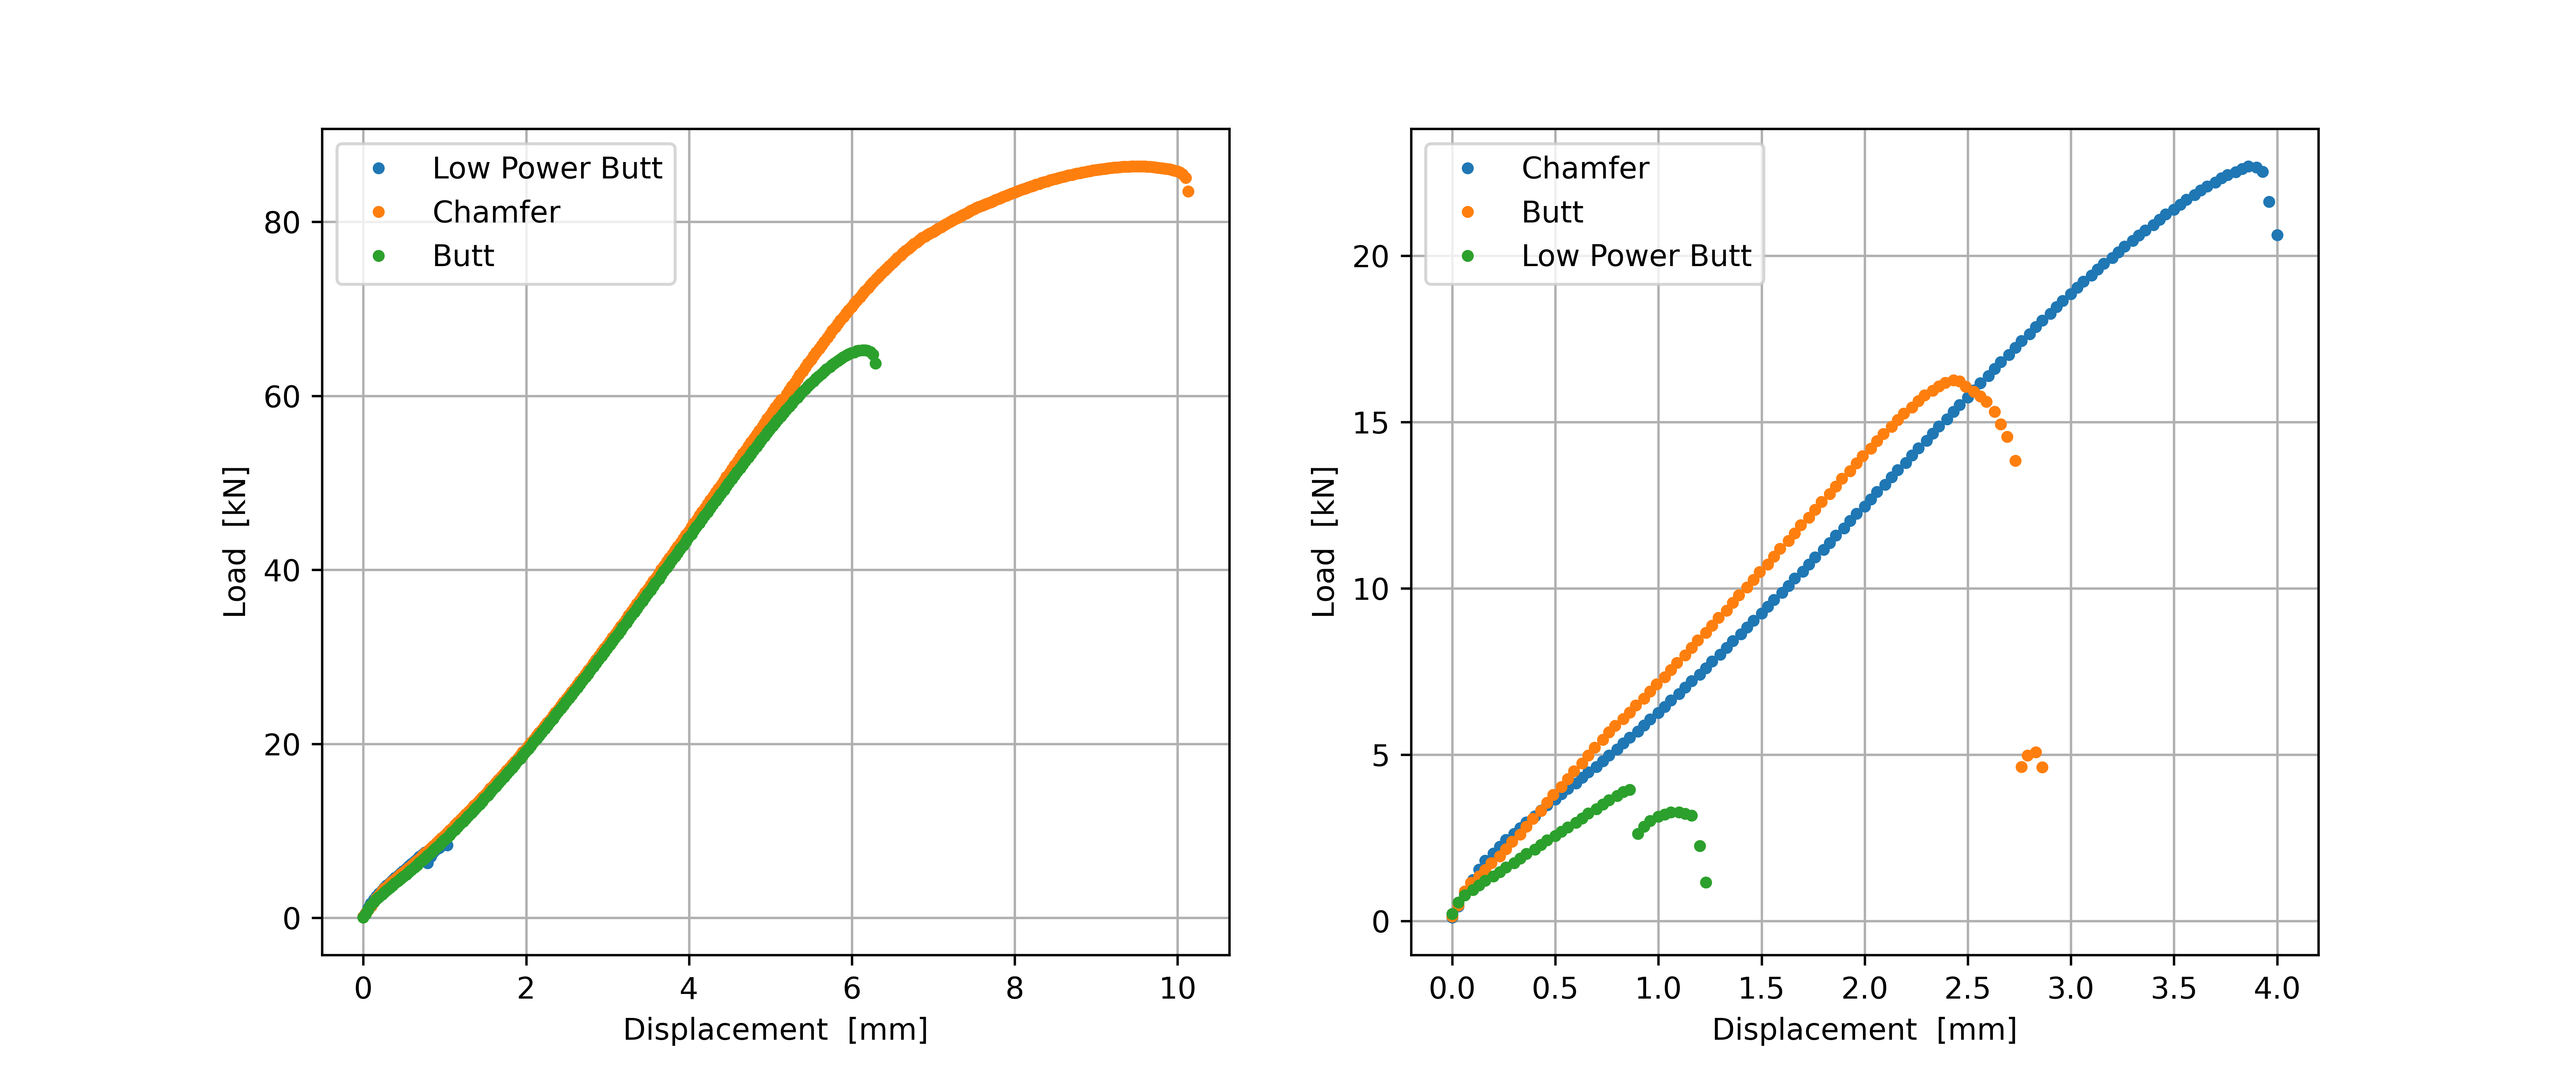
\includegraphics[width=\linewidth]{plots/q1-1018-6061.png}
    \caption{Load-Displacement curves of 1018 Steel (Left) and 6061 Aluminum (Right)}
    \label{fig:q1}
\end{figure}

We determined the strongest weld type to be Chamfer for both material types. Thus, we formed the stress-strain curve for this weld type for both materials. This is presented in Fig. \ref{fig:q2weld}. Proximally we constructed stress-strain curves for homogeneous non-welded 1018 Steel and 6061 Aluminum. These are presented in Fig. \ref{fig:q2norm}.
\begin{figure}[!hp!]
\begin{subfigure}{.5\textwidth}
    \centering
    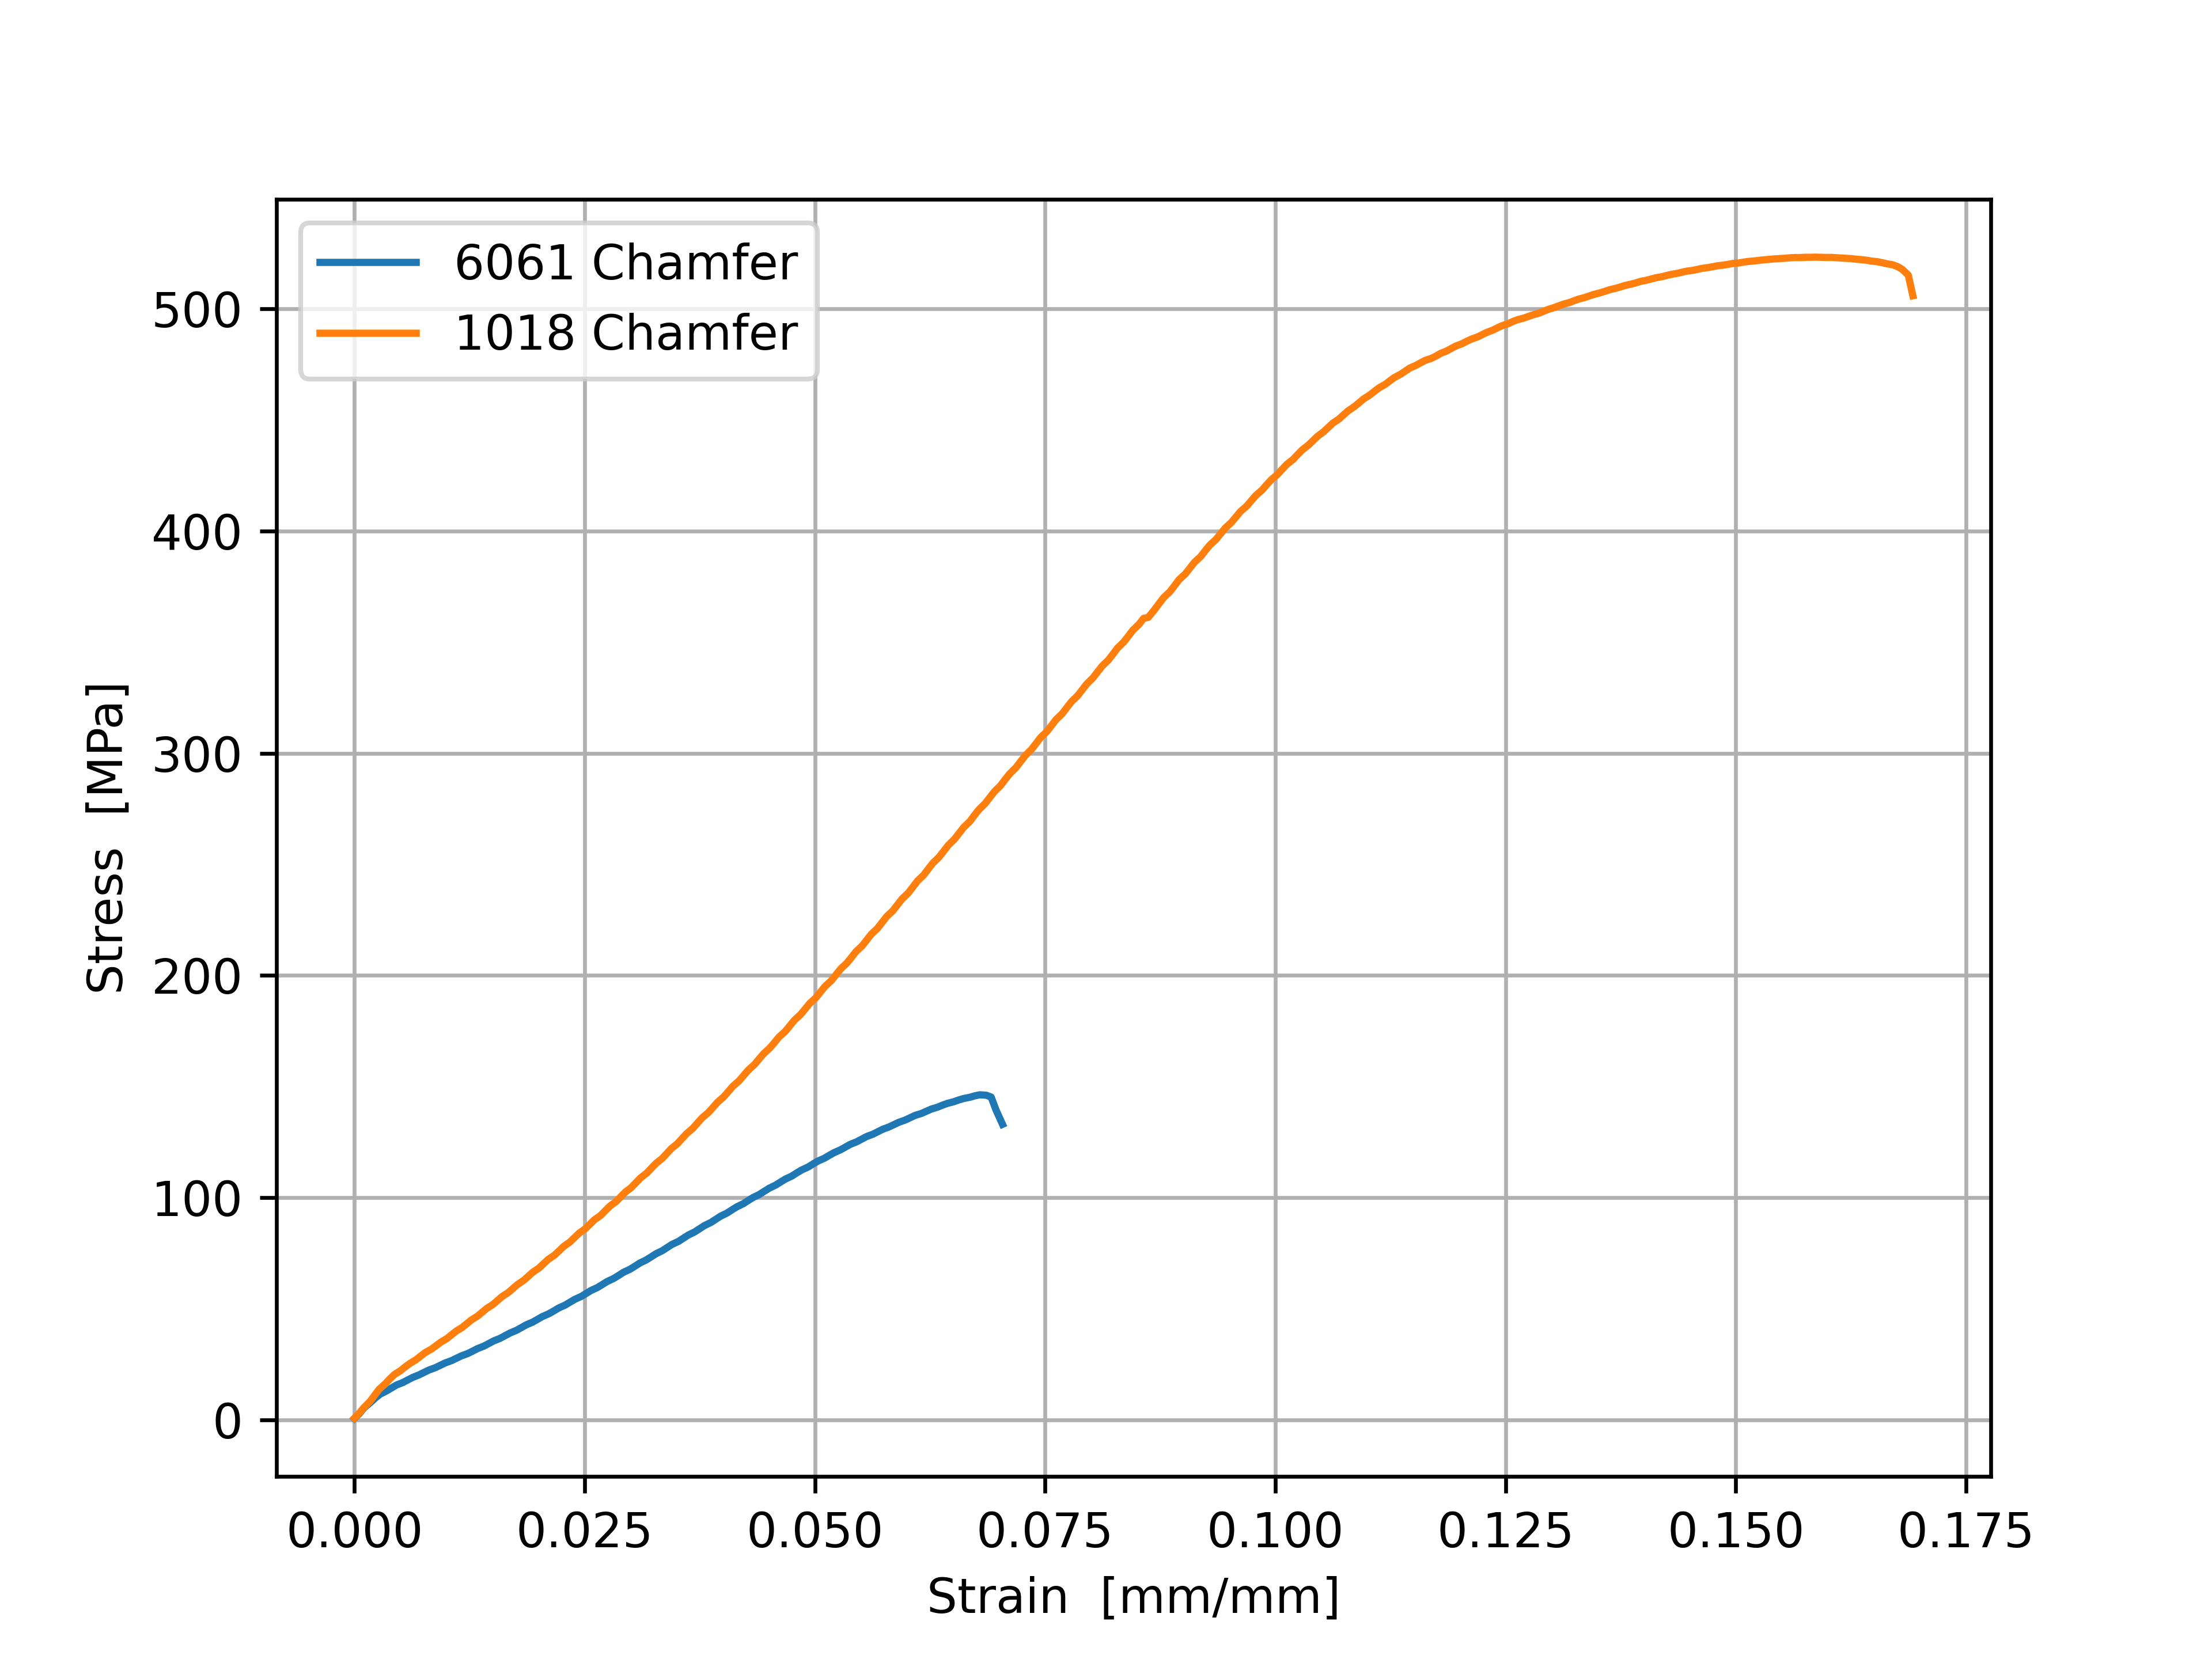
\includegraphics[width=\linewidth]{plots/q2weld.png}
    \caption{Stress-Strain Curves for Chamfer welded 1018 \newline \quad and 6061 specimens}
    \label{fig:q2weld}
\end{subfigure}
\begin{subfigure}{.5\textwidth}
    \centering
    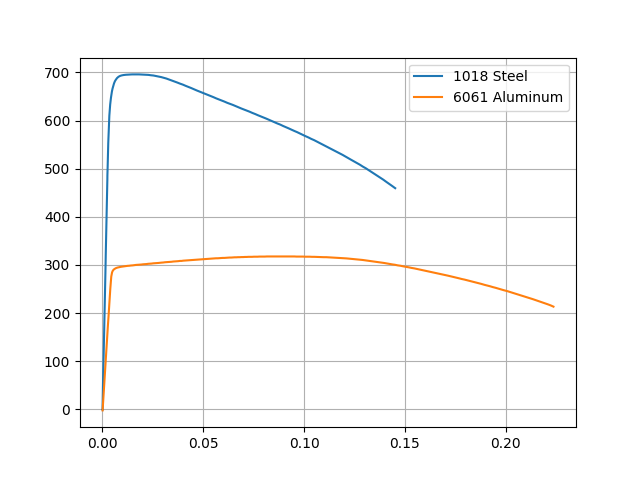
\includegraphics[width=\linewidth]{plots/q2norm.png}
    \caption{Stress-Strain Curves for 1018 and 6061  \newline \quad homogeneous specimens}
    \label{fig:q2norm}
\end{subfigure}
\end{figure}

\newpage
Further, from these curves we found the yield strength and ultimate tensile strength of each specimen. To determine the yield strength (UTS) we utilized the 0.2\% offset method. The results are presented in Tab. \ref{tab:q2lab7}

\begin{table}[!hp!]
    \centering
    \caption{Yield Strength and UTS of welded and homogeneous 1018 and 6061 specimens}
    \begin{tabular}{|c|c|c|c|c|}
        \toprule
        \bottomrule
        Material & 1018 Chamfer & 6061 Chamfer & 1018 Homogeneous & 6061 Homogeneous \\
        \toprule
        \bottomrule
        Yield Strength & 145.204 & 39.908 & 671.854 & 293.534 \\
        \hline
        UTS & 146.3 & 523.18 & 695.849 & 317.578 \\
        \hline
    \end{tabular}
    \label{tab:q2lab7}
\end{table}

Finally, we determined the Vickers hardness for the tested 1018 and 6061 specimens. We found the Vickers hardness as a function of the testing site, presented in Fig. \ref{fig:q4}. Each of the sub-plots has two vertical lines. To the left of the vertical lines is the base-metal region, between the lines is the heat effected region, and to the right is the fusion zone. Note, both plots have a 'Spline Interpolator', this is purely to aid in visualization of the overall trend of the data. Without these curves, the data is hard to visualize.  

\begin{figure}[!hp!]
    \centering
    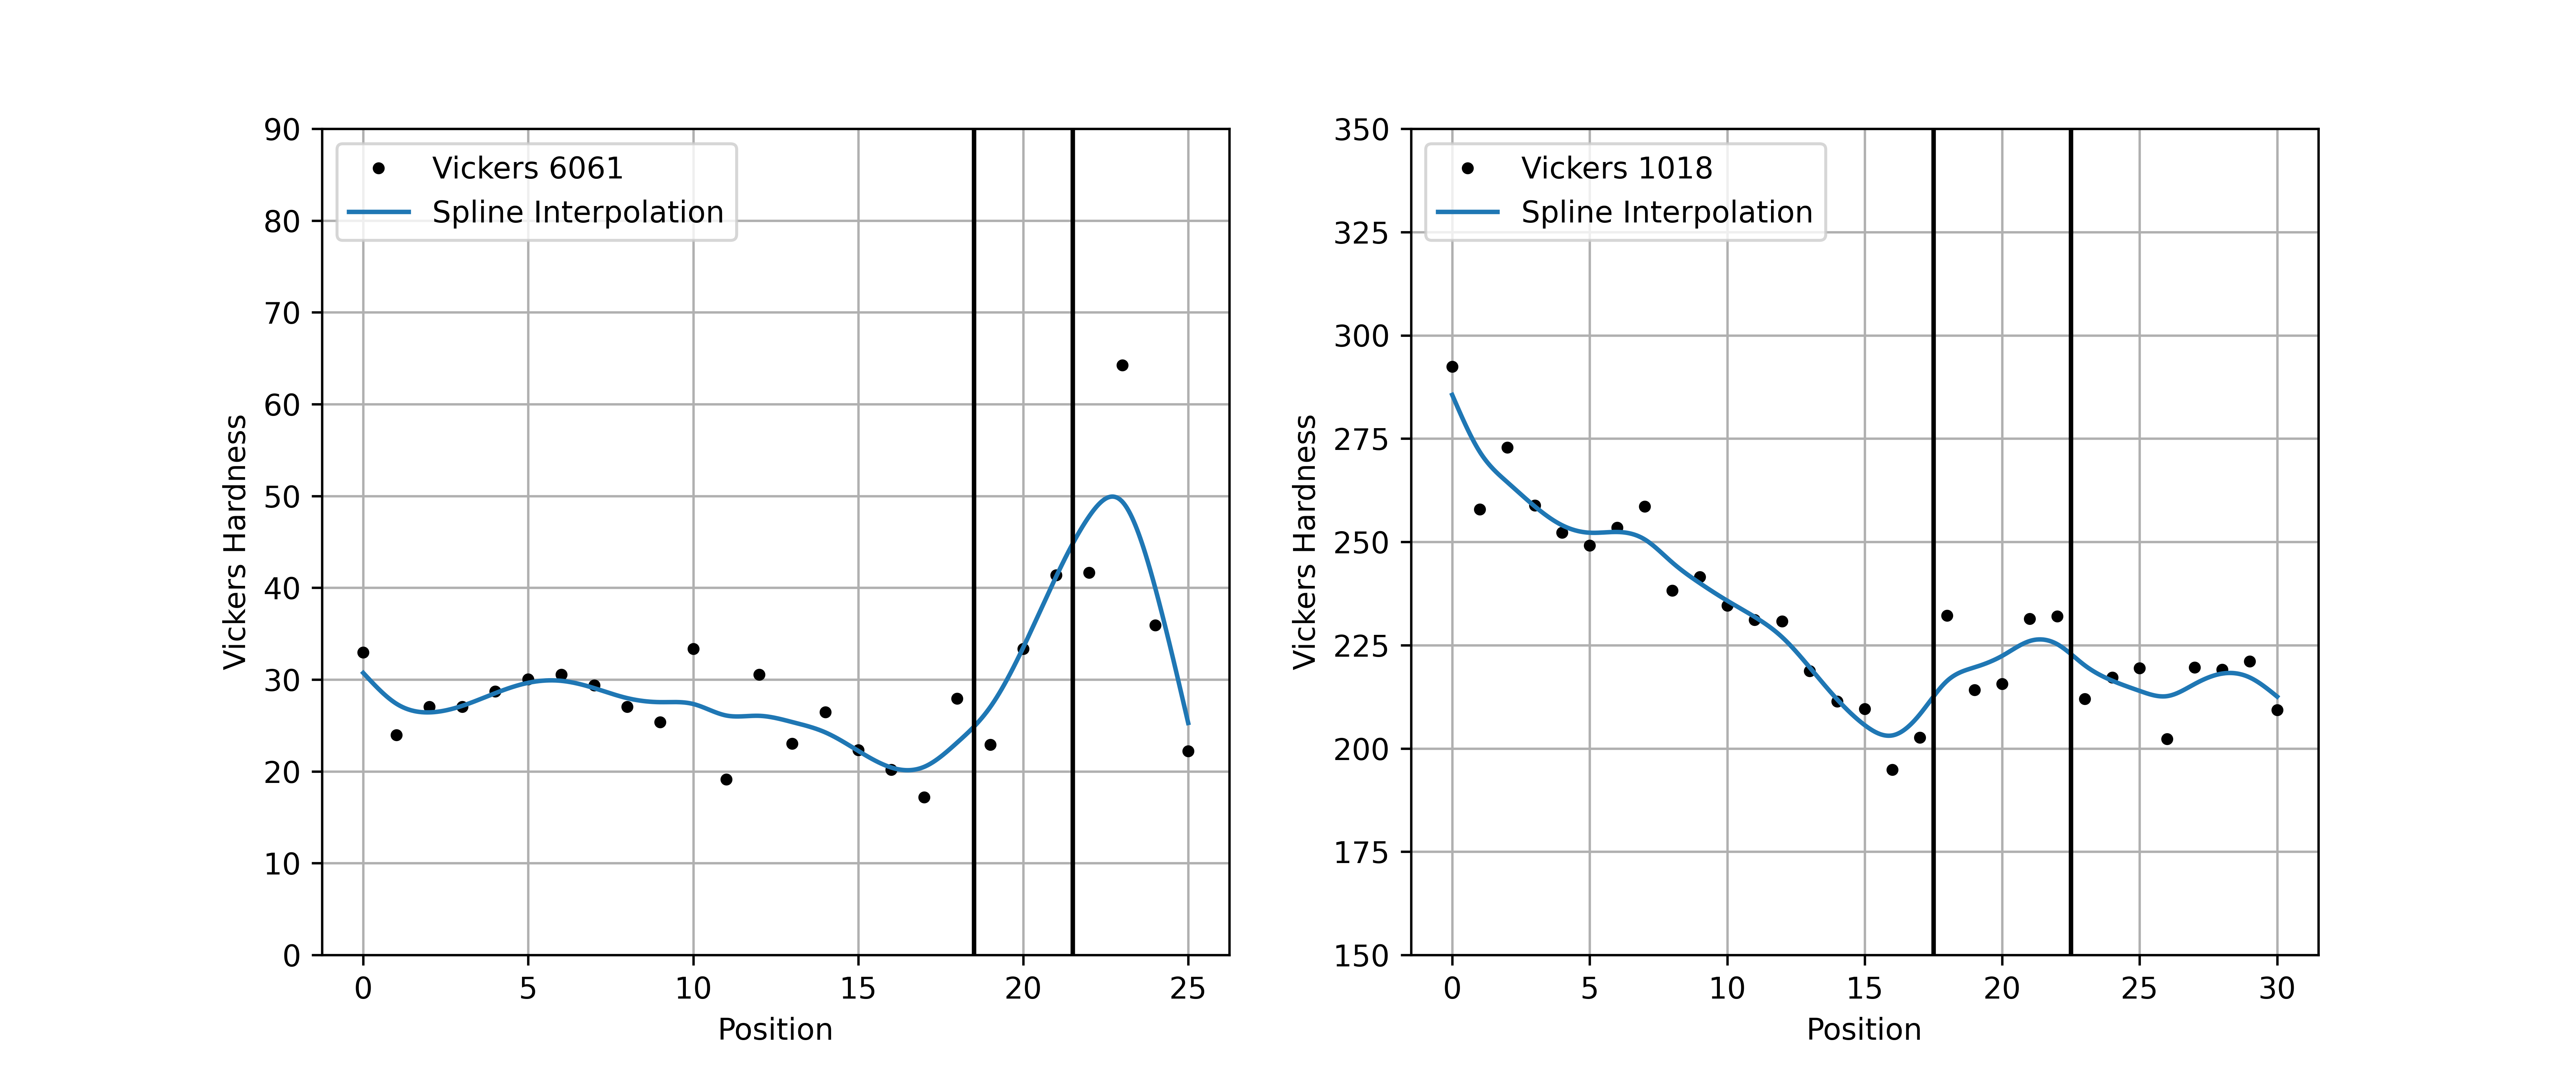
\includegraphics[width=\linewidth]{plots/q4.png}
    \caption{Vickers hardness for 6061 (Left) and 1018 (Right)}
    \label{fig:q4}
\end{figure}

\newpage
\section{Analysis and Discussion of Results}

\section{Answers to Questions}
To begin, we found the Load-Displacement curves of the three weld types for Aluminum 6061 and 1018 Steel. These curves are presented in Fig. \ref{fig:q1}. There is a clear impact of the weld type on the strength of each specimen. Noticeably the Low-Power Butt weld type was by far the weakest of the bunch. Thus, it can be determined that the lower the weld-power the weaker the weld is. Further, comparing the geometry of the welds, between Camfer and Butt, there is a clearly superior choice. The Camfer weld was superior in strength for both materials tested. 

Next, we found the stress-strain curves for the Camfer welded specimens as well as for standard homogeneous tensile specimens of the same material. These are presented in Figs. \ref{fig:q2weld} and \ref{fig:q2norm}. There is a clear distinction between the welded materials and their homogeneous counter-parts. First, the trend present in both of the welded materials is a small linear elastic region followed by a large pseudo-linear region of 'plastic' deformation. This pseudo-linear region is likely due to competing material properties between the weld material and the base material. The initial linear region is the stress region in which both sections of the specimen are elastically deforming, whereas the pseudo-linear region is where the base-material is elastically deforming and the weld-material is plastically deforming. Because of the competing deformations occurring, the yield strength of the welded materials was much lower than their homogeneous counterparts. Next, the impact of welding on the ductility of the specimens is less clear. For the 1018 specimen there was actually an increase in overall strain prior to fracture, whereas for the 6061 specimen there was a sharp decline. For both specimen however, there is a clear drop in overall toughness and also UTS. This inherently makes sense as less energy is going to deforming the material and more is going to separating the two regions. 

Next, we investigate two of the welded specimens. First, we will visually analyze the microstructure of each specimen. The format of each figure will be the same. On the left hand side of the figure is a macroscopic view of the specimen. Then on the right hand side, from the top to the bottom, is the fusion zone, the heat effected zone, and the base material. The microstructure for the Aluminum 6061 specimen is presented in Fig. \ref{fig:6061}, and the microstructure for the 1018 Steel is presented in Fig. \ref{fig:1018}.

\begin{figure}[!hp!]
    \centering
    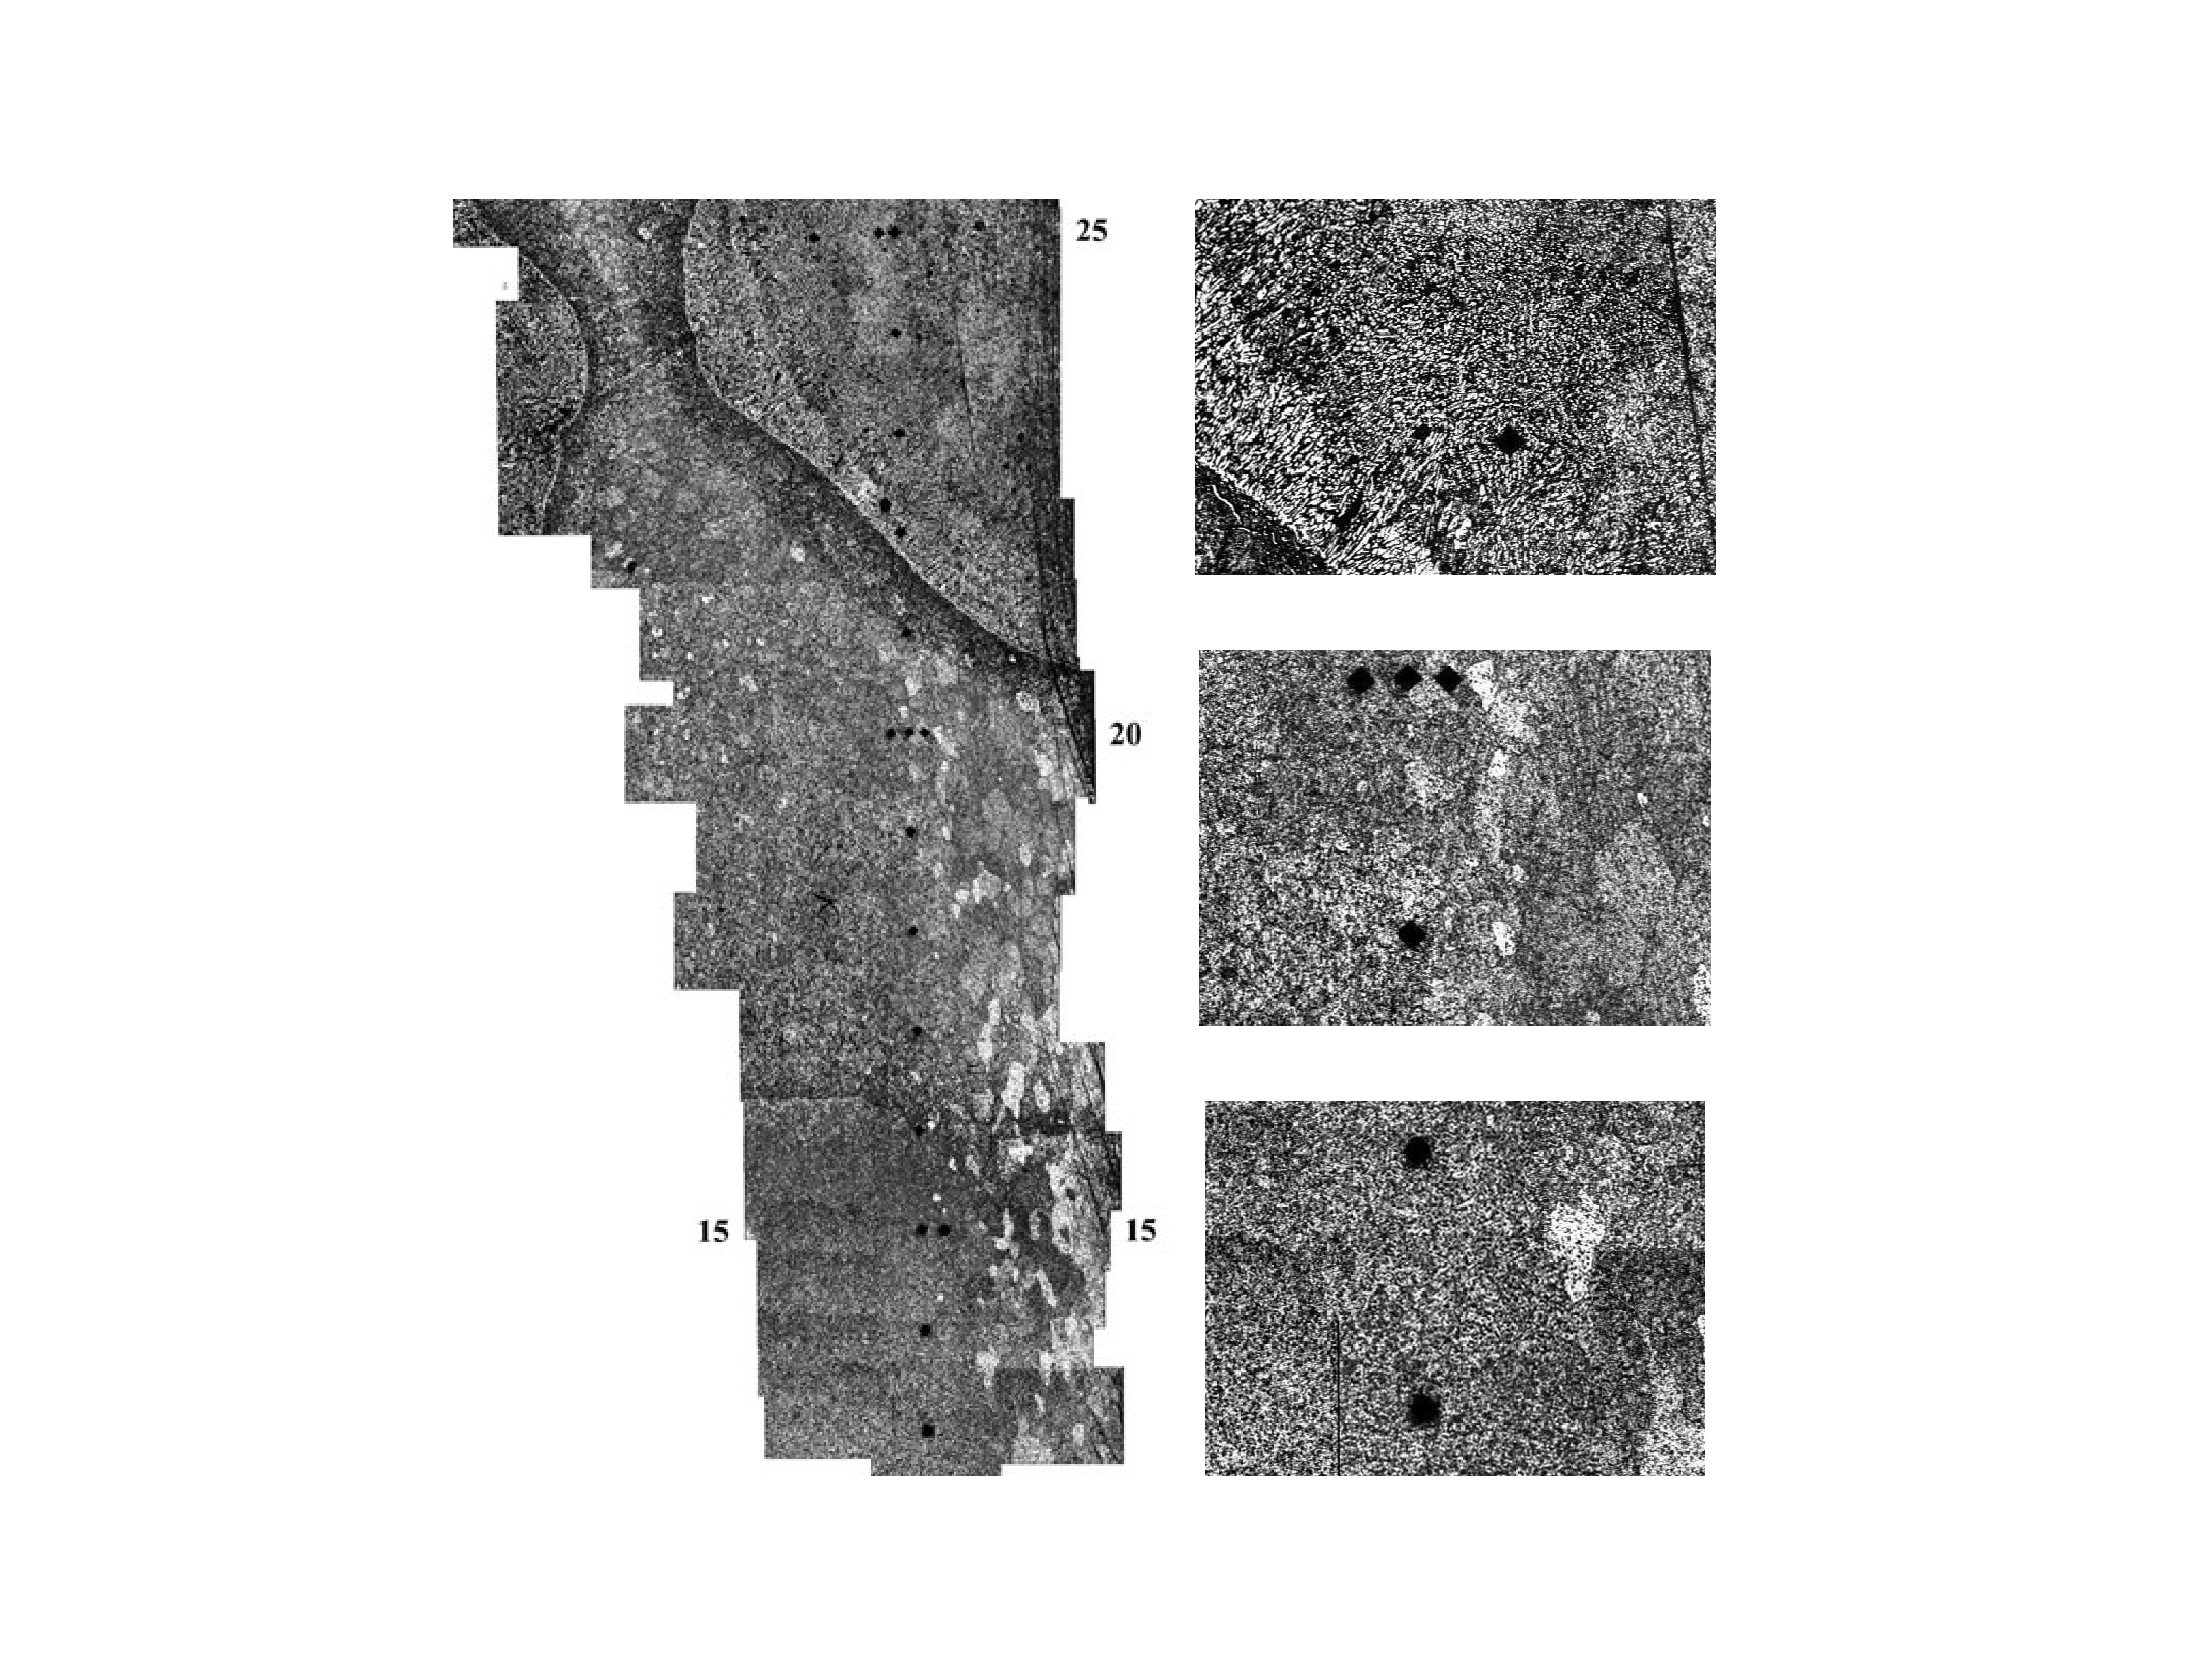
\includegraphics[width=1\linewidth]{plots/6061microcollage.png}
    \caption{Collage of microstructures of the Aluminum 6061 Specimen}
    \label{fig:6061}
\end{figure}
\begin{figure}[!hp!]
    \centering
    \includegraphics[width=1\linewidth]{plots/1018microcollage.png}
    \caption{Collage of microstructures of the 1018 Steel Specimen}
    \label{fig:1018}
\end{figure}

Finally, we determined the Vickers hardness at various locations on the 6061 and 1018 specimens. These results are presented in Fig. \ref{fig:q4}.
Welding has a clear impact on the hardness of each specimen. The closer to the welded region the stronger the variation from the expected hardness. In both heat affected regions, there is a localized increase in hardness closer to the fusion region. Further, in both cases there is an absolute minimum prior to the heat affected zone. This is likely due to a seepage of welding material into the base material ,at low quantities. This seepage would result in a large dislocation density locally increasing the hardness.

\section{Conclusions}

\section{References}

\printbibliography[heading = none]

\end{document}